\documentclass[twoside,12pt]{article}

\usepackage{dsctemplate}
\usepackage[margin=1in]{geometry}
\usepackage{amsmath}
\usepackage{amssymb,amsthm}
\usepackage{fancyhdr}
\usepackage{nicefrac}
\usepackage{minted}
\usetikzlibrary{quotes,angles,positioning,arrows.meta}
\usetikzlibrary{calc}
\usepackage{enumitem}
\usepackage{fancyvrb}
\usepackage{dirtytalk}
\usepackage{comment}

\DefineVerbatimEnvironment{verbatim}{Verbatim}{xleftmargin=.5in}

% configuration
% ------------------------------------------------------------------------------
% https://www.overleaf.com/project/651e1f6af0ac68cded0e43cf
% control whether solutions are shown or hidden
\showsolntrue

% page headers only on odd pages
\pagestyle{fancy}
\fancyhead{}
\fancyhead[RO]{PID: \rule{3in}{.5pt}}
\renewcommand{\headrulewidth}{0pt}
% \pagenumbering{gobble}

% ------------------------------------------------------------------------------

\begin{document}


\thispagestyle{empty}

\vspace{-5.5in}

\pstitle{%
    Quiz 2
}{DSC 10, Winter 2024}

\vspace{-.3in}

\begin{tabular}{rl}
    Full Name: & \inlineresponsebox[4in]{Solutions}\\
    PID: & \inlineresponsebox[4in]{A12345678}\vspace{.1in}\\
    Discussion: & \bubble{A (5PM)} \bubble{B (6PM)} \bubble{C (7PM)} \vspace{.3in} \\ 
\end{tabular}

\vspace{.1in}

\hline

\vspace{.1in}

\textbf{Instructions:}
    \begin{itemize}
        \item This quiz consists of 5 questions. You have a total of 20 minutes to complete it.
        \item Please write \textbf{clearly} in the provided answer boxes; we will not grade work that appears elsewhere. Completely fill in bubbles and square boxes; if we cannot tell which option(s) you selected, you may lose points.
        
            \bubble{A bubble means that you should only \textbf{select one choice}.}
            
            \squarebubble{A square box means you should \textbf{select all that apply}.}
        \item If your answer is a string, make sure to put it in quotes. If your answer is a float, make sure to include a decimal point.
        \item No aids are allowed (no notes, no calculators, and no computers).
    \end{itemize}

\vspace{.1in}

\hline

\vspace{2in}

\noindent By signing below, you are agreeing that you will behave honestly and fairly during
and after this quiz. 

\begin{tabular}{rl}
    \: \: \: \: \: Signature: & \inlineresponsebox[4in]{}\\
\end{tabular}

\vfill

\begin{center}
{\huge Version A} \vspace{.2in}

Please do not open your quiz until instructed to do so.

\end{center}

\newpage

\noindent The \texttt{laptops} DataFrame contains information on various factors that influence the pricing of laptops. Each row represents a laptop, and the columns are 
\begin{itemize}
    \item \texttt{"Mfr" (str)}: the company that manufactures the laptop, like \texttt{"Apple"} or \texttt{"Dell"}. \vspace{-0.1in}
    \item \texttt{"Model" (str)}: the model name of the laptop, such as \texttt{"MacBook Pro"}. \vspace{-0.1in}
    \item \texttt{"OS" (str)}: the operating system, such as \texttt{"macOS"} or \texttt{"Windows 11"}.
    \vspace{-0.1in}
    \item \texttt{"Screen Size" (float)}: the diagonal length of the screen, in inches.
    \vspace{-0.1in}
    \item \texttt{"Price" (float)}: the price of the laptop, in dollars.
\end{itemize}

\begin{probset}

\begin{prob}

We'd like to visualize the distribution of the \texttt{"Mfr"} column in the \texttt{laptops} DataFrame. Fill in the blanks so that the code below draws an appropriate plot.

\begin{verbatim}
laptops.groupby(__(a)__).__(b)__.get([__(c)__]).plot(kind=__(d)__)
\end{verbatim}

\texttt{a}: \inlineresponsebox[3in]{\texttt{"Mfr"}}{}, \texttt{b}: \inlineresponsebox[3in]{\texttt{count()}}{}

\texttt{c}: \inlineresponsebox[3in]{\texttt{"Model"}, \texttt{"OS"}, \texttt{"Screen Size"}, or \texttt{"Price"}}{}, \texttt{d}: \inlineresponsebox[3in]{\texttt{"bar"} or \texttt{"barh"}}{}

\end{prob}

\begin{prob}
Fill in the blanks so that \texttt{rotten\_apple} evaluates to the number of laptops manufactured by \texttt{"Apple"} that are priced below the median price of all laptops.

\begin{verbatim}
x = __(a)__
y = __(b)__
rotten_apple = laptops[x __(c)__ y].__(d)__
\end{verbatim}

\texttt{a}: \biginlineresponsebox[6.36in]{\texttt{laptops.get("Mfr") == "Apple"}}{}

\texttt{b}: \biginlineresponsebox[6.36in]{\texttt{laptops.get("Price") < laptops.get("Price").median()}}{}

\texttt{c}: \inlineresponsebox[3in]{\texttt{\&}}{}, \texttt{d}: \inlineresponsebox[3in]{\texttt{shape[0]}}{}
\end{prob}

\newpage

\begin{prob}

Select all the true statements below.

\squarebubble{When you set the index of a DataFrame, the specified column becomes the index, and \\\hspace*{0.25in}the old index becomes a column.}

\correctsquarebubble{After grouping a DataFrame, the resulting number of rows is less than or equal to the \\\hspace*{0.25in}original number of rows.}

\correctsquarebubble{The area of a density histogram is always equal to 1.}

%\squarebubble{Histograms shows the distribution of a categorical variable.}

\squarebubble{A scatter plot has one numerical axis and one categorical axis.}

%\correctsquarebubble{It is possible to draw a histogram from a DataFrame that contains just one numerical column.}

\squarebubble{The height of the tallest bar in a density histogram is always less than 1.}

%\squarebubble{After grouping a DataFrame, the index of remains unchanged}.

\end{prob}

\begin{prob}

A density histogram of \texttt{"Screen Size"} is shown below.

\vspace{-0.2in}
\begin{minipage}[t]{4.25in}
\noindent 
\begin{center}
    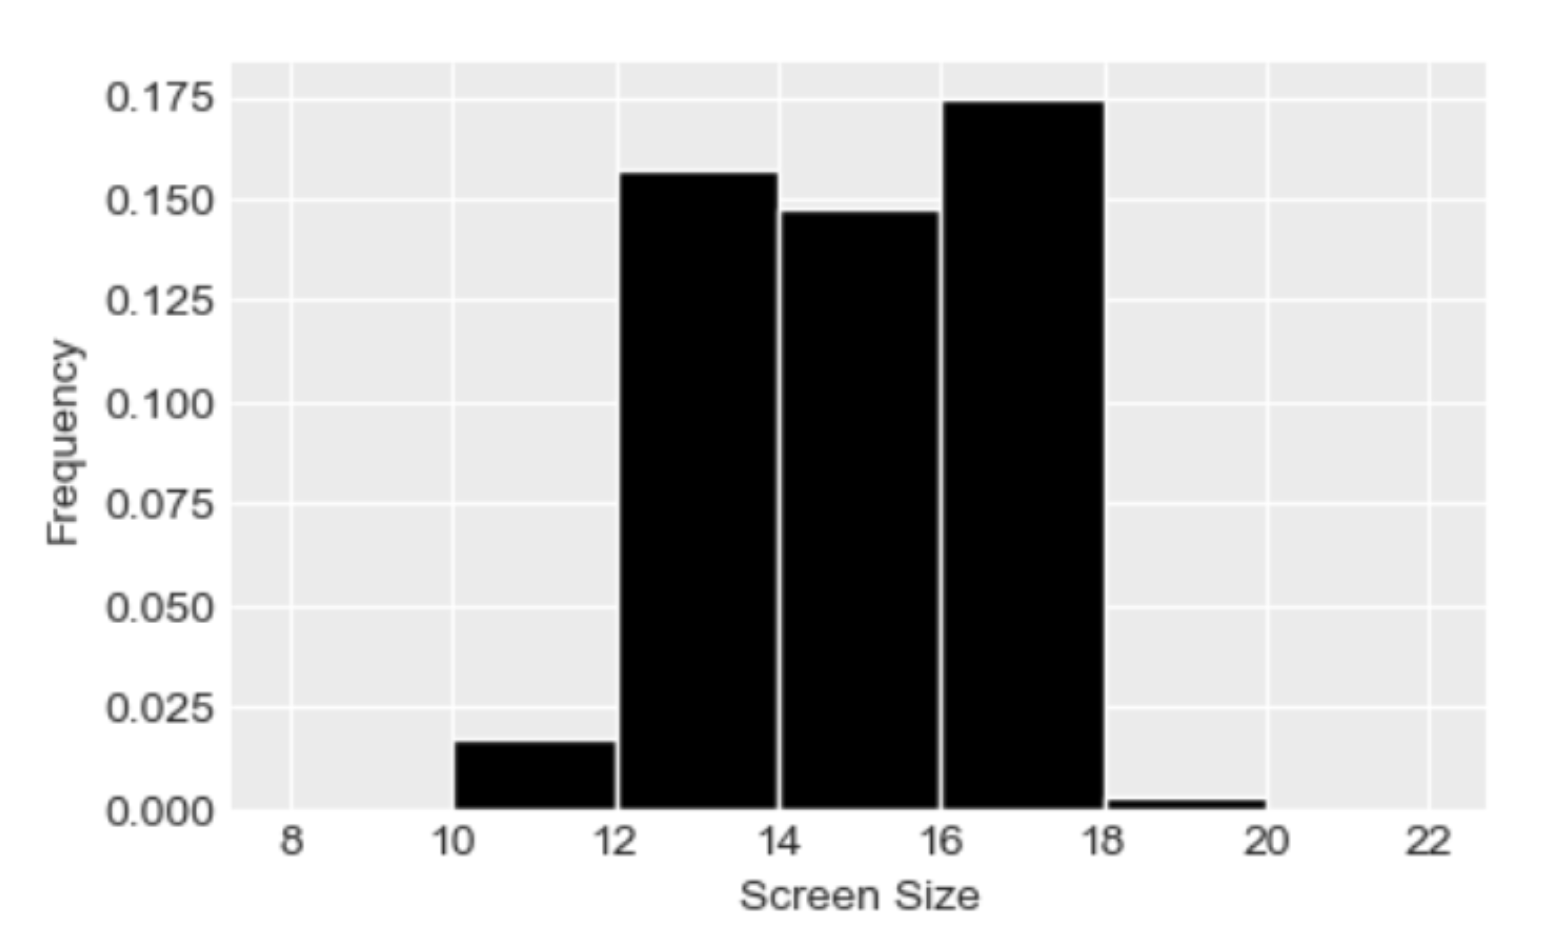
\includegraphics[width=\textwidth]{quiz_images/histogram.png}   
\end{center}
\end{minipage} \hspace{0.25in}
\begin{minipage}[t]{2.25in}
\vspace{0.3in}
\noindent What \textbf{percentage} of computer models have a \texttt{"Screen Size"} of at least 16 inches but less than 18 inches? Give your answer as an integer rounded to the \textbf{nearest multiple of 5}.

\begin{center}
\tikz[baseline=-.5em]{
        \node[
            draw, rectangle, inner sep=0, text centered, minimum height=3em, 
            text width=1in, align=center
        ] at (0,0) {
            \phantom{8888888}\%

        };
        \useasboundingbox 
            ([shift={(1mm,1mm)}]current bounding box.north east)
            rectangle 
            ([shift={(-1mm,-1mm)}]current bounding box.south west);
    }%
\end{center}

\end{minipage}

\end{prob}
\vspace{-0.2in}
\begin{prob}
\vspace{-0.1in}
\begin{subprobset}
\begin{subprob}
\textbf{Using \texttt{groupby}}, write an expression that evaluates to the average price of laptops with the \texttt{"macOS"} operating system.

\begin{responsebox}{0.75in}      
   \texttt{laptops.groupby("OS").mean().get("Price").loc["macOS"]}
\end{responsebox}
\end{subprob}
\begin{subprob}
\textbf{Without using \texttt{groupby}}, write an expression that evaluates to the average price of laptops with the \texttt{"macOS"} operating system (the same quantity as above).

\begin{responsebox}{0.75in}
    \texttt{laptops[laptops.get("OS") == "macOS"].get("Price").mean()}
\end{responsebox}
\end{subprob}
\end{subprobset}

\end{prob}

\end{probset}

\newpage

\begin{center}
\textbf{Before submitting your quiz, make sure your PID is on the front page and on the top right corner of page 3.}
\end{center}

\end{document}

% save for next time

\begin{prob}
What does the following expression represent:  
\begin{center}
    \texttt{items.shape[0] * items.shape[1]}
\end{center}

\bubble{The total number of columns in the DataFrame}

\bubble{The sum of the elements in the DataFrame}

\bubble{The total number of rows in the DataFrame}

\bubble{The total number of elements in the DataFrame}

\end{prob}